\documentclass{beamer}

\mode<presentation>

\usepackage[dutch]{babel}
%\usepackage{beamerthemesplit}
\usepackage{hyperref}

\usetheme{Berlin}
\useinnertheme{rounded}
\usecolortheme{rose}
\setbeamertemplate{navigation symbols}{} 
\title{Design patterns}
\author{W. Oele}
\date{\today}

\begin{document}
\frame{\titlepage}

\section{Design patterns}

\begin{frame}
\frametitle{Deze les}
\begin{itemize}
\item Het strategy patroon
\item Het bridge patroon
\end{itemize}
\end{frame}

\section{Strategy}
\begin{frame} \frametitle{Het strategy pattern}
  \begin{itemize}
  \item naam: het strategy pattern
  \item doel: algoritmen runtime kunnen inzetten
  \item hoe: implementatie van algoritmen scheiden van selectie 
  \item gevolgen: alle algoritmen moeten dezelfde interface hebben
  \end{itemize}
\end{frame}


\begin{frame}
\frametitle{Het strategy pattern}
\begin{itemize}
\item Een timmerman moet twee stukken hout aan elkaar vastmaken.
\item Hij doet dat met een hamer en spijkers.
\end{itemize}
\begin{center}
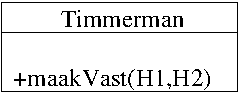
\includegraphics[width=4cm]{timmer1}
\end{center}
\end{frame}

\begin{frame}[fragile]
\frametitle{Het strategy pattern}
\begin{verbatim}
public class Timmerman
{
public Constructie maakVast(H1, H2)
   {
      ...
      timmeren met hamer en spijkers;
      ...
      return constructie;
   }
}
\end{verbatim}
\end{frame}

\begin{frame}
\frametitle{Het strategy pattern}
Sommige constructies worden \emph{niet} met hamer en spijkers gemaakt:
\begin{itemize}
\item houtlijm
\end{itemize}
\begin{center}
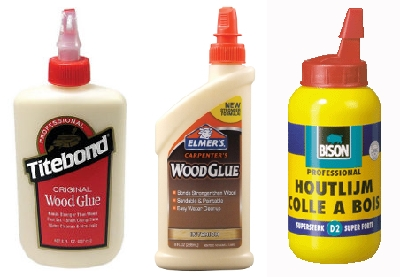
\includegraphics[width=5cm]{houtlijm}
\end{center}
\end{frame}

\begin{frame}
\frametitle{Een poging}
\begin{center}
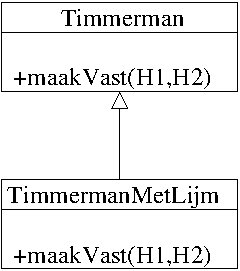
\includegraphics[width=4cm]{timmer2}
\end{center}
\end{frame}


\begin{frame}[fragile]
\frametitle{Een poging}
\begin{verbatim}
public class TimmermanMetLijm extends Timmerman
{
   public Constructie maakVast(H1, H2)
   {
      ...
      stukken hout vastmaken met lijm ;
      ...
      return constructie;
   }
}
\end{verbatim}
\end{frame}
\begin{frame}
\frametitle{Het strategy pattern}
Sommige constructies worden \emph{niet} met hamer en spijkers gemaakt:
\begin{itemize}
\item bouten en moeren
\end{itemize}
\begin{center}
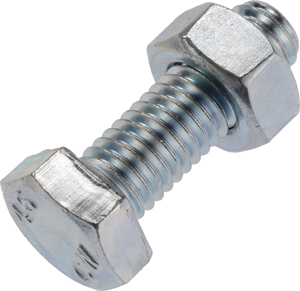
\includegraphics[width=3cm]{bout}
\end{center}
\end{frame}

\begin{frame}
\frametitle{Een poging}
\begin{center}
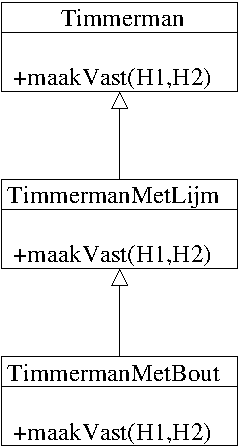
\includegraphics[width=3cm]{timmer3}
\end{center}
\end{frame}

\begin{frame}
\frametitle{Het strategy pattern}
Sommige constructies worden \emph{niet} met hamer en spijkers gemaakt:
\begin{itemize}
\item schroeven
\end{itemize}
\begin{center}
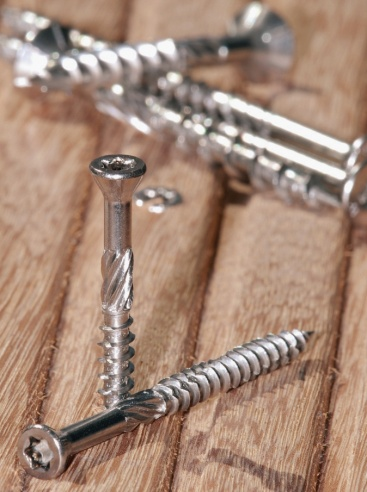
\includegraphics[width=3cm]{schroef}
\end{center}
\end{frame}

\begin{frame}
\frametitle{Het strategy pattern}
Sommige constructies worden \emph{niet} met hamer en spijkers gemaakt:
\begin{itemize}
\item deuvels
\end{itemize}
\begin{center}
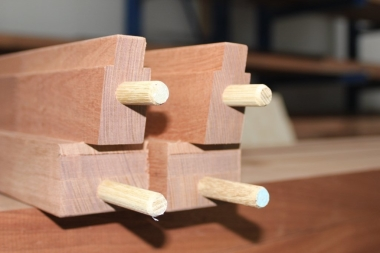
\includegraphics[width=5cm]{deuvel}
\end{center}
\end{frame}

\begin{frame}
\frametitle{Het strategy pattern}
Mogelijke manieren om twee stukken hout te verbinden:
\begin{itemize}
\item spijkers
\item houtlijm
\item bouten en moeren
\item schroeven
\item deuvels
\end{itemize}
\end{frame}

\begin{frame}
\frametitle{Het strategy pattern}
\begin{itemize}
\item Voorgaande manier van ontwerpen leidt tot een lange keten van afgeleide klassen.
\item Niet fraai
\item Foutgevoelig
\end{itemize}
\end{frame}

\begin{frame}
\frametitle{Het strategy pattern}
\begin{itemize}
\item Een timmerman kan, naast 2 stukken hout aan elkaar vast maken, veel meer doen.
\item Het afleiden van allerlei timmermannen is derhalve niet handig.
\end{itemize}
\begin{center}
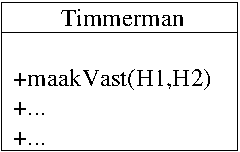
\includegraphics[width=4cm]{timmer4}
\end{center}
\end{frame}

\begin{frame}
\frametitle{Het strategy pattern}
\begin{itemize}
\item Wat varieert is iedere keer het aan elkaar vast maken van twee stukken hout.
\item We kapselen dit in in een aparte klasse:
\end{itemize}
\begin{center}
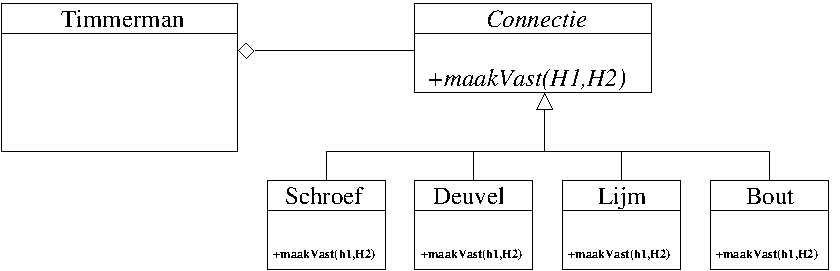
\includegraphics[width=10cm]{timmer5}
\end{center}
\emph{``Find what varies and encapsulate it\ldots''}
\end{frame}

\begin{frame}
\frametitle{Het strategy pattern: algemeen}
\begin{center}
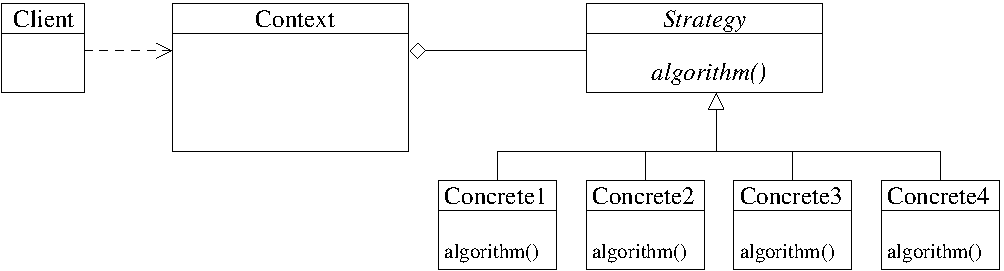
\includegraphics[width=10cm]{strategy1}
\end{center}
\end{frame}

\begin{frame}
\frametitle{Richtlijnen}
\begin{itemize}
\item Find what varies and encapsulate it.
\item Denk over een klasse in termen van verantwoordelijkheden:
  \begin{itemize}
  \item Wie is verantwoordelijk voor wat?
  \item Teveel verantwoordelijkheid? $\rightarrow$ opsplitsen 
  \end{itemize}
\end{itemize}
\end{frame}

\section{Bridge}
\begin{frame} \frametitle{Het bridge pattern}
  \begin{itemize}
  \item naam: het bridge patroon
  \item doel: decoupling: implementaties scheiden van abstractie
  \item hoe: interface ontwerpen voor alle afgeleide klassen
  \item gevolgen: 
    \begin{itemize}
    \item clients weten niets van implementatie
    \item verbeterde uitbreidbaarheid
    \item geen combinatorische explosies
    \end{itemize}
  \end{itemize}
\end{frame}

\begin{frame}
\frametitle{Het probleem}
Een machine produceert verschillende soorten glaswerk:
\begin{itemize}
\item erlenmeyer
\item maatcylinder
\item kolf
\item fles
\item maatbeker
\item etc.
\end{itemize}\pause
Elk van deze soorten dient voorzien te worden van:
\begin{itemize}
\item opdruk
\item graveerwerk
\item stickers
\end{itemize}\pause
Ook voor het graveerwerk hebben we een machine\ldots
\end{frame}

\begin{frame}
\frametitle{Glaswerk(1)}
\begin{center}
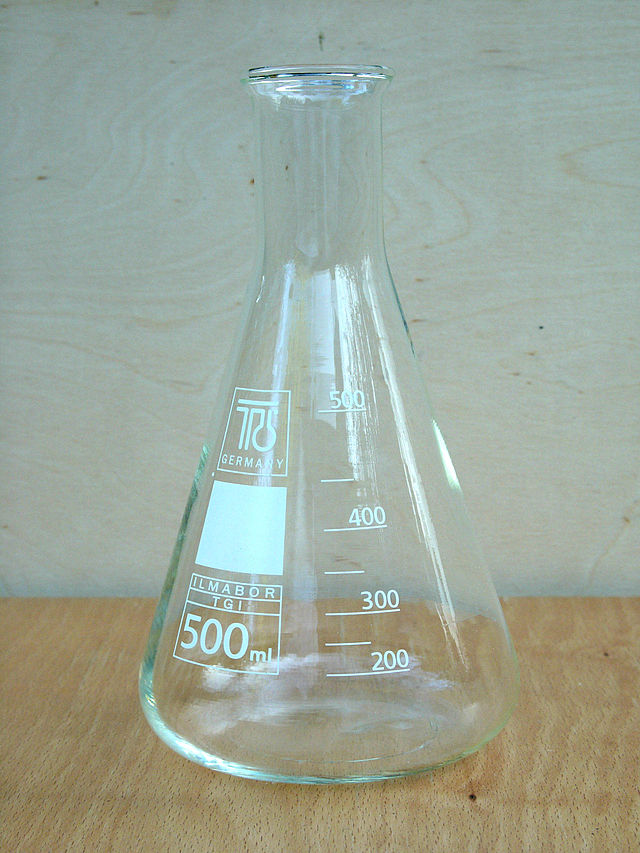
\includegraphics[width=4cm]{erlenm}
\end{center}
\end{frame}

\begin{frame}
\frametitle{Glaswerk(2)}
\begin{center}
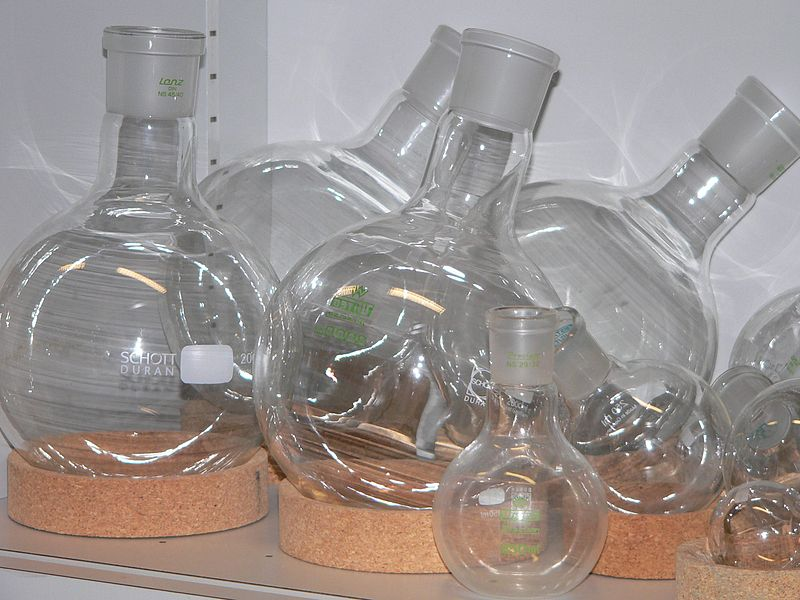
\includegraphics[width=7cm]{kolf}
\end{center}
\end{frame}

\begin{frame}
\frametitle{Het model: poging 1}
\begin{center}
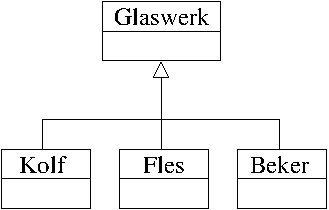
\includegraphics[width=5cm]{bridge1}
\end{center}
\end{frame}

\begin{frame}
\frametitle{Het model: poging 1}
\begin{center}
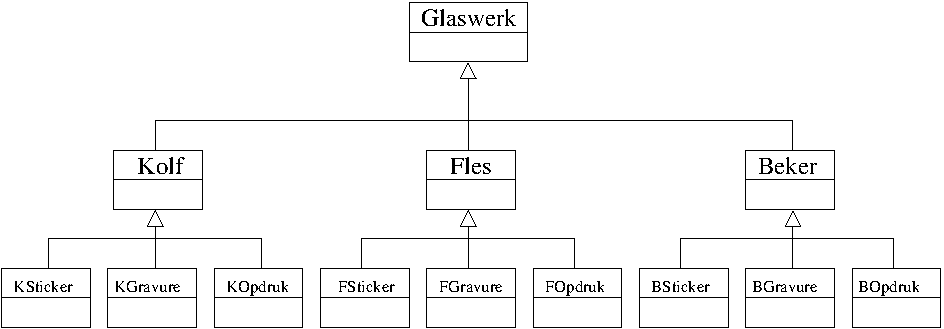
\includegraphics[width=11cm]{bridge2}
\end{center}
Slechts drie soorten glaswerk en drie soorten tekst: 13 klassen!
\end{frame}

\begin{frame}
\frametitle{Het model: poging 2}
\begin{center}
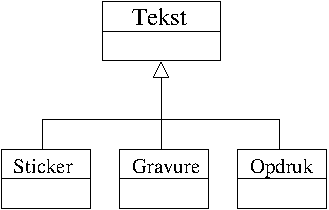
\includegraphics[width=5cm]{bridge3}
\end{center}
\end{frame}

\begin{frame}
\frametitle{Het model: poging 2}
\begin{center}
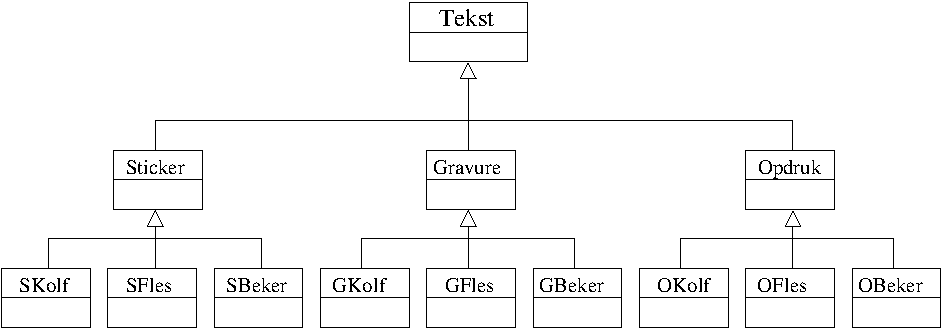
\includegraphics[width=11cm]{bridge4}
\end{center}
Slechts drie soorten tekst en drie soorten glaswerk: opnieuw 13 klassen!
\end{frame}


\begin{frame}
\frametitle{Het bridge pattern}
Welke abstracties zitten er in het probleem?\pause
\begin{itemize}
\item verschillende soorten glaswerk:
  \begin{itemize}
  \item kolf, fles, beker,\ldots
  \end{itemize}\pause
\item verschillende manieren om ``iets'' op het glas te krijgen:
  \begin{itemize}
  \item sticker, gravure, opdruk,\ldots
  \end{itemize}
\end{itemize}
\end{frame}

\begin{frame}
\frametitle{Het bridge pattern}
\begin{center}
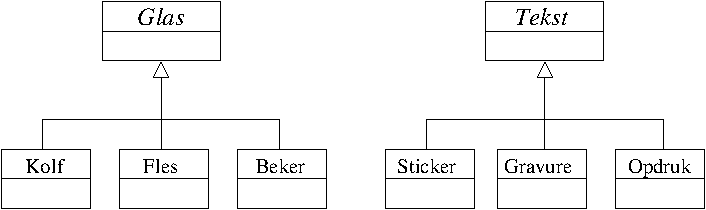
\includegraphics[width=10cm]{bridge5}
\end{center}
\end{frame}

\begin{frame}
\frametitle{Het bridge pattern}
Wat hebben beide abstracties met elkaar te maken?\pause
\begin{itemize}
\item Een tekst heeft een glas om op te staan?
\item Een glas heeft een tekst die er op \'e\'en of andere manier op gezet is.
\end{itemize}
\end{frame}


\begin{frame}
\frametitle{Het bridge pattern}
\begin{center}
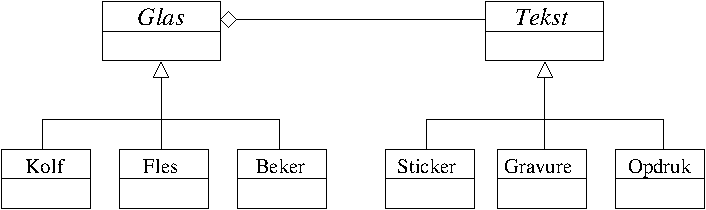
\includegraphics[width=10cm]{bridge6}
\end{center}
\end{frame}


\begin{frame}[fragile]
\frametitle{Het bridge pattern}
\begin{verbatim}
public abstract class Glas
{
   protected Tekst tekst;
   public abstract void plaatsTekst(String s);

   public Glas(Tekst t)
   {
      tekst=t;
   }

}
\end{verbatim}
\end{frame}

\begin{frame}
\frametitle{Het bridge pattern algemeen}
\begin{center}
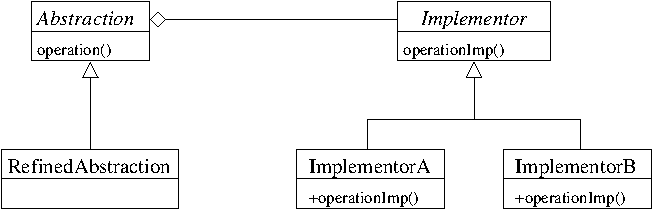
\includegraphics[width=10cm]{bridge7}
\end{center}
\end{frame}

\end{document}